\documentclass[aspectratio=169,10pt]{beamer}

% ====================
% Theme and Colors
% ====================
\usetheme{Madrid}
\usecolortheme{default}

% JP Morgan-inspired color scheme
\definecolor{jpmblue}{RGB}{0, 51, 102}
\definecolor{jpmlightblue}{RGB}{0, 118, 186}
\definecolor{jpmgray}{RGB}{128, 128, 128}
\definecolor{jpmaccent}{RGB}{0, 150, 136}
\definecolor{lightbg}{RGB}{245, 248, 250}

\setbeamercolor{palette primary}{bg=jpmblue,fg=white}
\setbeamercolor{palette secondary}{bg=jpmlightblue,fg=white}
\setbeamercolor{palette tertiary}{bg=jpmblue,fg=white}
\setbeamercolor{structure}{fg=jpmblue}
\setbeamercolor{title}{fg=white,bg=jpmblue}
\setbeamercolor{frametitle}{fg=white,bg=jpmblue}
\setbeamercolor{block title}{bg=jpmlightblue,fg=white}
\setbeamercolor{block body}{bg=lightbg,fg=black}
\setbeamercolor{block title alerted}{bg=red!70!black,fg=white}
\setbeamercolor{block body alerted}{bg=red!5,fg=black}
\setbeamercolor{block title example}{bg=jpmaccent,fg=white}
\setbeamercolor{block body example}{bg=jpmaccent!5,fg=black}
\setbeamercolor{item}{fg=jpmlightblue}

\setbeamertemplate{navigation symbols}{}
\setbeamertemplate{footline}{
  \leavevmode%
  \hbox{%
    \begin{beamercolorbox}[wd=.33\paperwidth,ht=2.5ex,dp=1ex,center]{palette primary}%
      \usebeamerfont{author in head/foot}\insertshortauthor
    \end{beamercolorbox}%
    \begin{beamercolorbox}[wd=.34\paperwidth,ht=2.5ex,dp=1ex,center]{palette secondary}%
      \usebeamerfont{title in head/foot}\insertshorttitle
    \end{beamercolorbox}%
    \begin{beamercolorbox}[wd=.33\paperwidth,ht=2.5ex,dp=1ex,right]{palette primary}%
      \insertframenumber{} / \inserttotalframenumber\hspace*{2ex}
    \end{beamercolorbox}}%
}

% ====================
% Packages
% ====================
\usepackage{amsmath,amssymb,amsthm}
\usepackage{graphicx}
\usepackage{booktabs}
\usepackage{array}
\usepackage{tikz}
\usetikzlibrary{arrows.meta,positioning,shapes.geometric,calc,fit,decorations.pathreplacing}
\usepackage{algorithm}
\usepackage{algorithmic}
\usepackage{multirow}
\usepackage{xcolor}
\usepackage{hyperref}

% ====================
% Custom Commands
% ====================
\newcommand{\E}{\mathbb{E}}
\newcommand{\R}{\mathbb{R}}
\newcommand{\N}{\mathcal{N}}
\newcommand{\argmin}{\operatorname*{arg\,min}}
\newcommand{\tr}{\operatorname{tr}}
\newcommand{\highlight}[1]{\textcolor{jpmlightblue}{\textbf{#1}}}
\newcommand{\remark}[1]{\textcolor{jpmaccent}{\textit{#1}}}

% ====================
% Title Information
% ====================
\title[Particle Flow \& Differentiable PF]{Particle Flow Filter and\\Differentiable Particle Filter}
\subtitle{JP Morgan MLCOE TSRL 2026 Internship --- Question 2}
\author{Haokai Huang}
\date{\today}
\institute{}

\begin{document}

% ============================================================
% TITLE SLIDE
% ============================================================
\begin{frame}[plain]
\titlepage
\end{frame}

% ============================================================
% OUTLINE
% ============================================================
\begin{frame}{Outline}
\begin{columns}[T]
\begin{column}{0.48\textwidth}
\textbf{Part 1: Classical $\to$ Particle Flows}
\begin{itemize}
  \item State Space Models
  \item KF, EKF, UKF, Particle Filter
  \item EDH / LEDH Particle Flow
  \item PF-PF Framework (Li \& Coates 2017)
\end{itemize}
\vspace{0.5em}
\textbf{Part 2: Advanced Methods}
\begin{itemize}
  \item Stochastic Particle Flow (Dai 2022)
  \item Optimal Homotopy \& Stiffness Mitigation
  \item Differentiable Particle Filter
  \item OT Resampling (Sinkhorn)
\end{itemize}
\end{column}
\begin{column}{0.48\textwidth}
\textbf{Bonus 1: HMC vs PMMH}
\begin{itemize}
  \item Differentiable PF enables HMC
  \item 3$\times$ efficiency gain over PMMH
\end{itemize}
\vspace{0.5em}
\textbf{Bonus 2: Neural OT Acceleration}
\begin{itemize}
  \item mGradNet, FNO, DeepONet
  \item 50--60$\times$ speedup potential
\end{itemize}
\vspace{0.5em}
\textbf{Bonus 3: Neural State-Space LSTM}
\begin{itemize}
  \item Gaussian \& Topical SSL
  \item DPF-HMC vs Particle Gibbs
\end{itemize}
\end{column}
\end{columns}
\end{frame}


% ============================================================
% PART 1
% ============================================================
\section{Part 1: From Classical Filters to Particle Flows}

% ---------- SSM ----------
\begin{frame}{State Space Models (SSMs)}
\begin{block}{General Formulation}
\vspace{-0.5em}
\begin{align}
  \text{State:} \quad x_t &= f(x_{t-1}) + w_t, \quad w_t \sim \N(0, Q) \\
  \text{Observation:} \quad y_t &= h(x_t) + v_t, \quad v_t \sim \N(0, R)
\end{align}
\end{block}

\textbf{Goal:} Compute the posterior $p(x_t \mid y_{1:t})$ sequentially.

\vspace{0.5em}
\begin{columns}[T]
\begin{column}{0.48\textwidth}
\begin{exampleblock}{Linear-Gaussian (LGSSM)}
\begin{itemize}
  \item $f(x) = Fx$, $h(x) = Hx$
  \item Kalman Filter is \highlight{optimal} (MMSE)
  \item Exact closed-form posterior
\end{itemize}
\end{exampleblock}
\end{column}
\begin{column}{0.48\textwidth}
\begin{alertblock}{Nonlinear / Non-Gaussian}
\begin{itemize}
  \item Closed-form posterior unavailable
  \item Must approximate: EKF, UKF, PF
  \item Challenge: particle degeneracy
\end{itemize}
\end{alertblock}
\end{column}
\end{columns}
\end{frame}

% ---------- KF ----------
\begin{frame}{Kalman Filter: Joseph-Stabilized Form}
\begin{columns}[T]
\begin{column}{0.55\textwidth}
\textbf{Predict:}
\vspace{-0.5em}
\begin{align}
  \hat{x}_{t|t-1} &= F \hat{x}_{t-1|t-1} \\
  P_{t|t-1} &= F P_{t-1|t-1} F^\top + Q
\end{align}

\textbf{Update:}
\vspace{-0.5em}
\begin{align}
  K_t &= P_{t|t-1} H^\top (H P_{t|t-1} H^\top + R)^{-1}
\end{align}

\begin{block}{Joseph Stabilized Covariance}
\vspace{-0.5em}
\[
  P_{t|t} = (I - K_t H) P_{t|t-1} (I - K_t H)^\top + K_t R K_t^\top
\]
\end{block}
\remark{$\Rightarrow$ Guarantees symmetry \& positive-definiteness}
\end{column}
\begin{column}{0.42\textwidth}
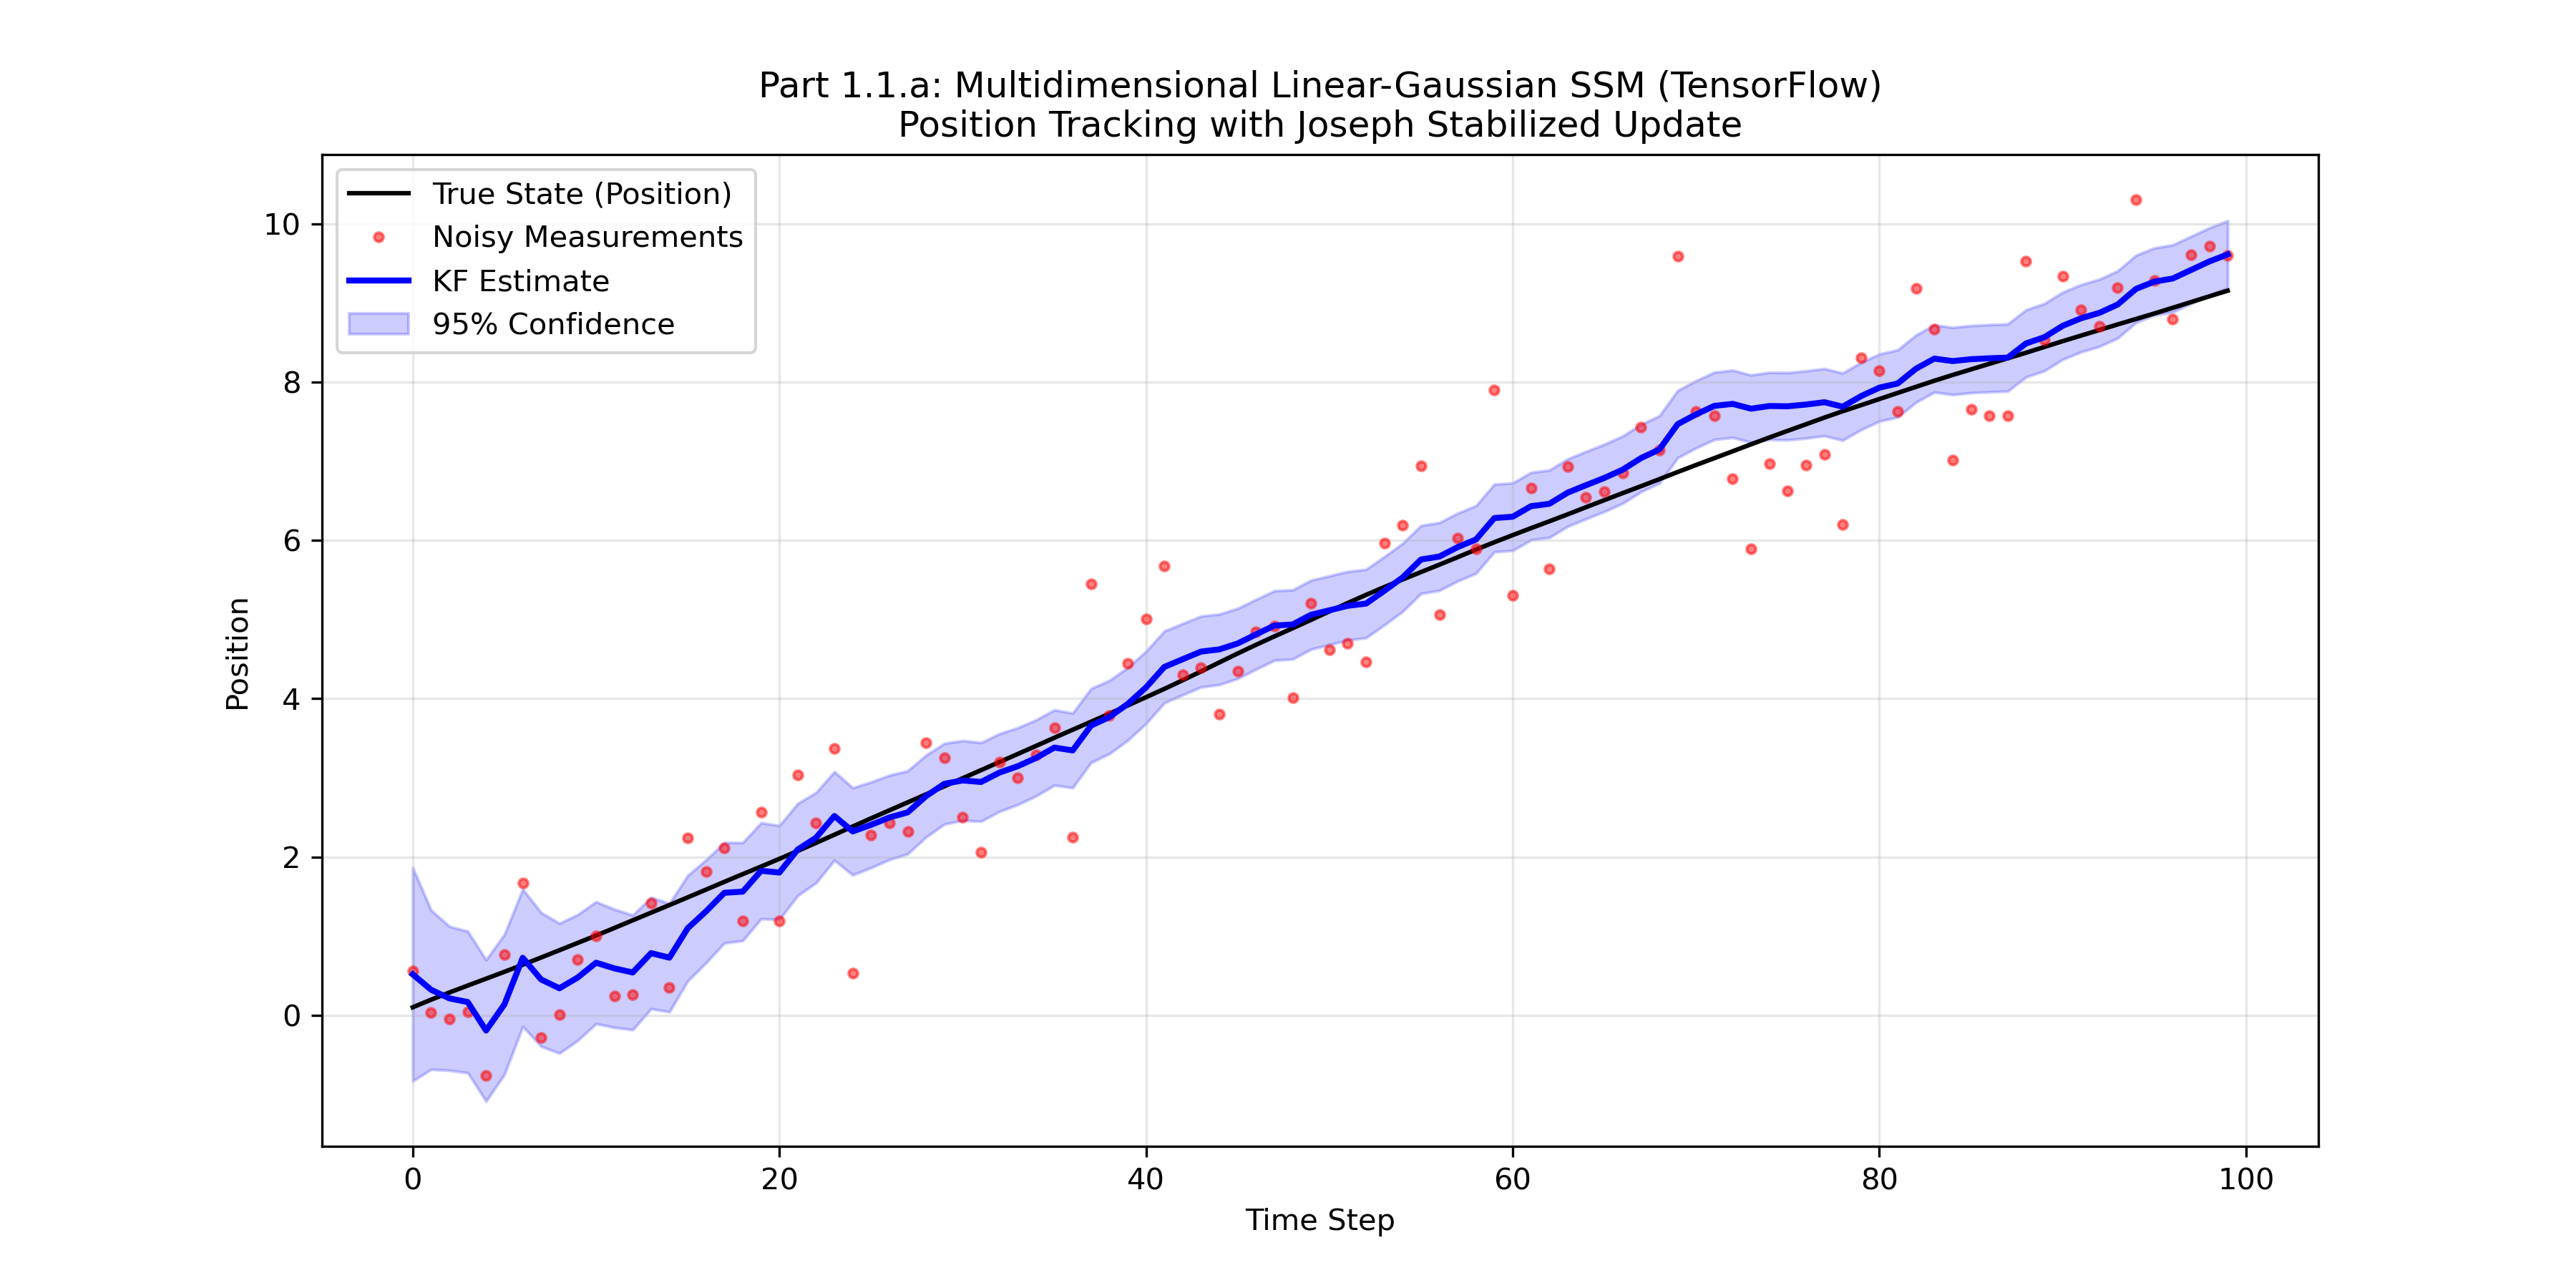
\includegraphics[width=\textwidth]{../results/run_kalman_filter.png}
\vspace{-0.5em}
{\scriptsize KF tracking on 2D LGSSM. Well-calibrated 95\% CI.}
\end{column}
\end{columns}
\end{frame}

% ---------- SV Model ----------
\begin{frame}{Test Problem: Stochastic Volatility Model}
\begin{columns}[T]
\begin{column}{0.55\textwidth}
\begin{block}{SV Model (Doucet 2009)}
\textbf{State:}
\vspace{-0.5em}
\[
  x_t = 0.91 \cdot x_{t-1} + \sigma_v \cdot v_t
\]
\textbf{Observation:}
\vspace{-0.5em}
\[
  y_t = 0.5 \cdot \exp(x_t / 2) \cdot w_t
\]
\end{block}

\vspace{0.3em}
\textbf{Why challenging?}
\begin{itemize}
  \item Observation noise variance $\propto \exp(x_t)$: \highlight{highly nonlinear}
  \item EKF linearization fails for large $|x_t|$
  \item UKF sigma points can collapse
  \item State-dependent heteroscedasticity
\end{itemize}
\end{column}
\begin{column}{0.42\textwidth}
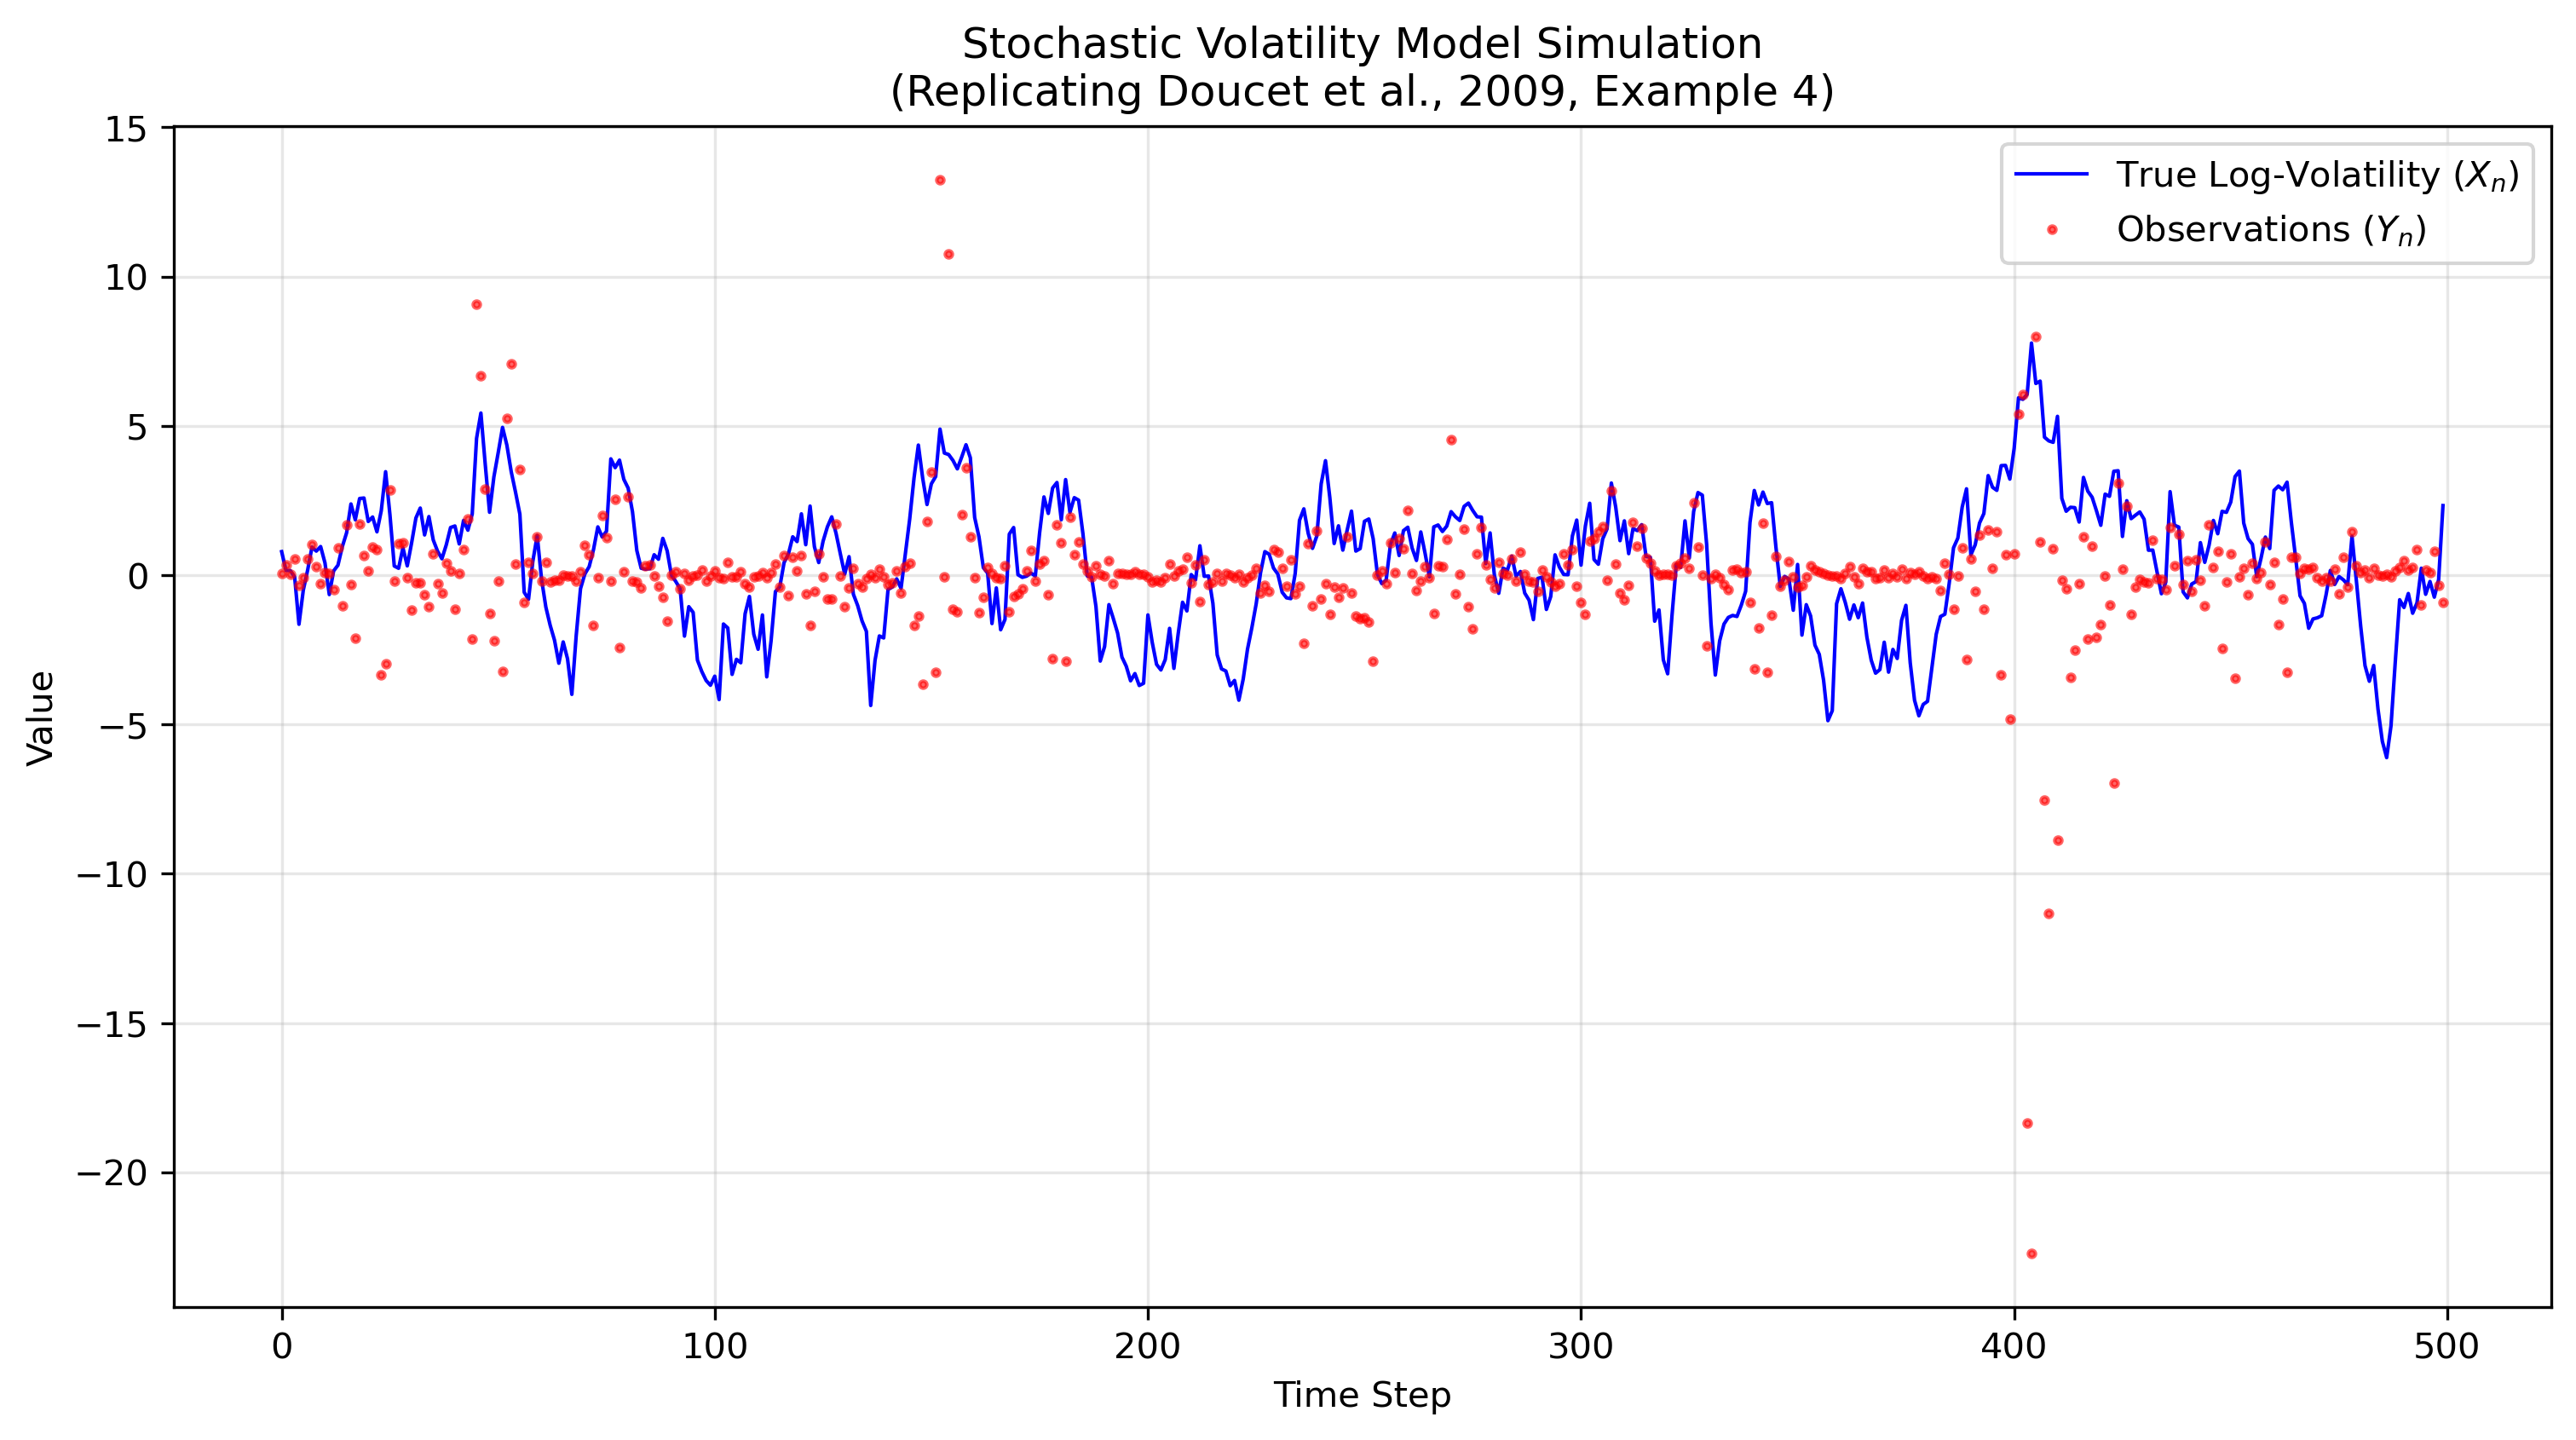
\includegraphics[width=\textwidth]{../results/sv_model_simulation.png}
\vspace{-0.5em}
{\scriptsize Latent log-volatility $x_t$ (blue) and heteroscedastic observations $y_t$ (red dots).}
\end{column}
\end{columns}
\end{frame}

% ---------- EKF / UKF ----------
\begin{frame}{EKF and UKF: Approximate Nonlinear Filtering}
\begin{columns}[T]
\begin{column}{0.48\textwidth}
\begin{block}{Extended Kalman Filter}
\begin{itemize}
  \item Linearize via Taylor expansion:
    \[
      F_t = \left.\frac{\partial f}{\partial x}\right|_{\hat{x}_{t-1}}, \quad
      H_t = \left.\frac{\partial h}{\partial x}\right|_{\hat{x}_t}
    \]
  \item \highlight{AutoDiff Jacobians} via TF \texttt{GradientTape}
  \item First-order accuracy
\end{itemize}
\end{block}
\remark{Fails on SV model: exponential $h(x)$ $\Rightarrow$ large linearization error}
\end{column}
\begin{column}{0.48\textwidth}
\begin{block}{Unscented Kalman Filter}
\begin{itemize}
  \item Propagate $2n+1$ \highlight{sigma points}:
    \[
      \chi_i \to f(\chi_i), \quad h(\chi_i)
    \]
  \item Recover mean/cov from weighted points
  \item Second-order accuracy, \textbf{no Jacobians}
\end{itemize}
\end{block}
\remark{Better than EKF but still Gaussian assumption}
\end{column}
\end{columns}
\end{frame}

% ---------- PF ----------
\begin{frame}{Particle Filter: Bootstrap SIR}
\begin{columns}[T]
\begin{column}{0.55\textwidth}
\begin{block}{Algorithm}
\begin{enumerate}
  \item \textbf{Predict:} $x_t^{(i)} \sim p(x_t \mid x_{t-1}^{(i)})$
  \item \textbf{Weight:} $w_t^{(i)} \propto p(y_t \mid x_t^{(i)})$
  \item \textbf{Estimate:} $\hat{x}_t = \sum_i w_t^{(i)} x_t^{(i)}$
  \item \textbf{Resample} when ESS $< N/2$
\end{enumerate}
\end{block}

\vspace{0.3em}
\textbf{Effective Sample Size:}
\[
  \text{ESS} = \frac{1}{\sum_{i=1}^N (w_t^{(i)})^2}
\]

\remark{ESS drops below $N/10$ within 20 steps on SV model}

\vspace{0.3em}
Key challenge: \highlight{particle degeneracy}
\end{column}
\begin{column}{0.42\textwidth}
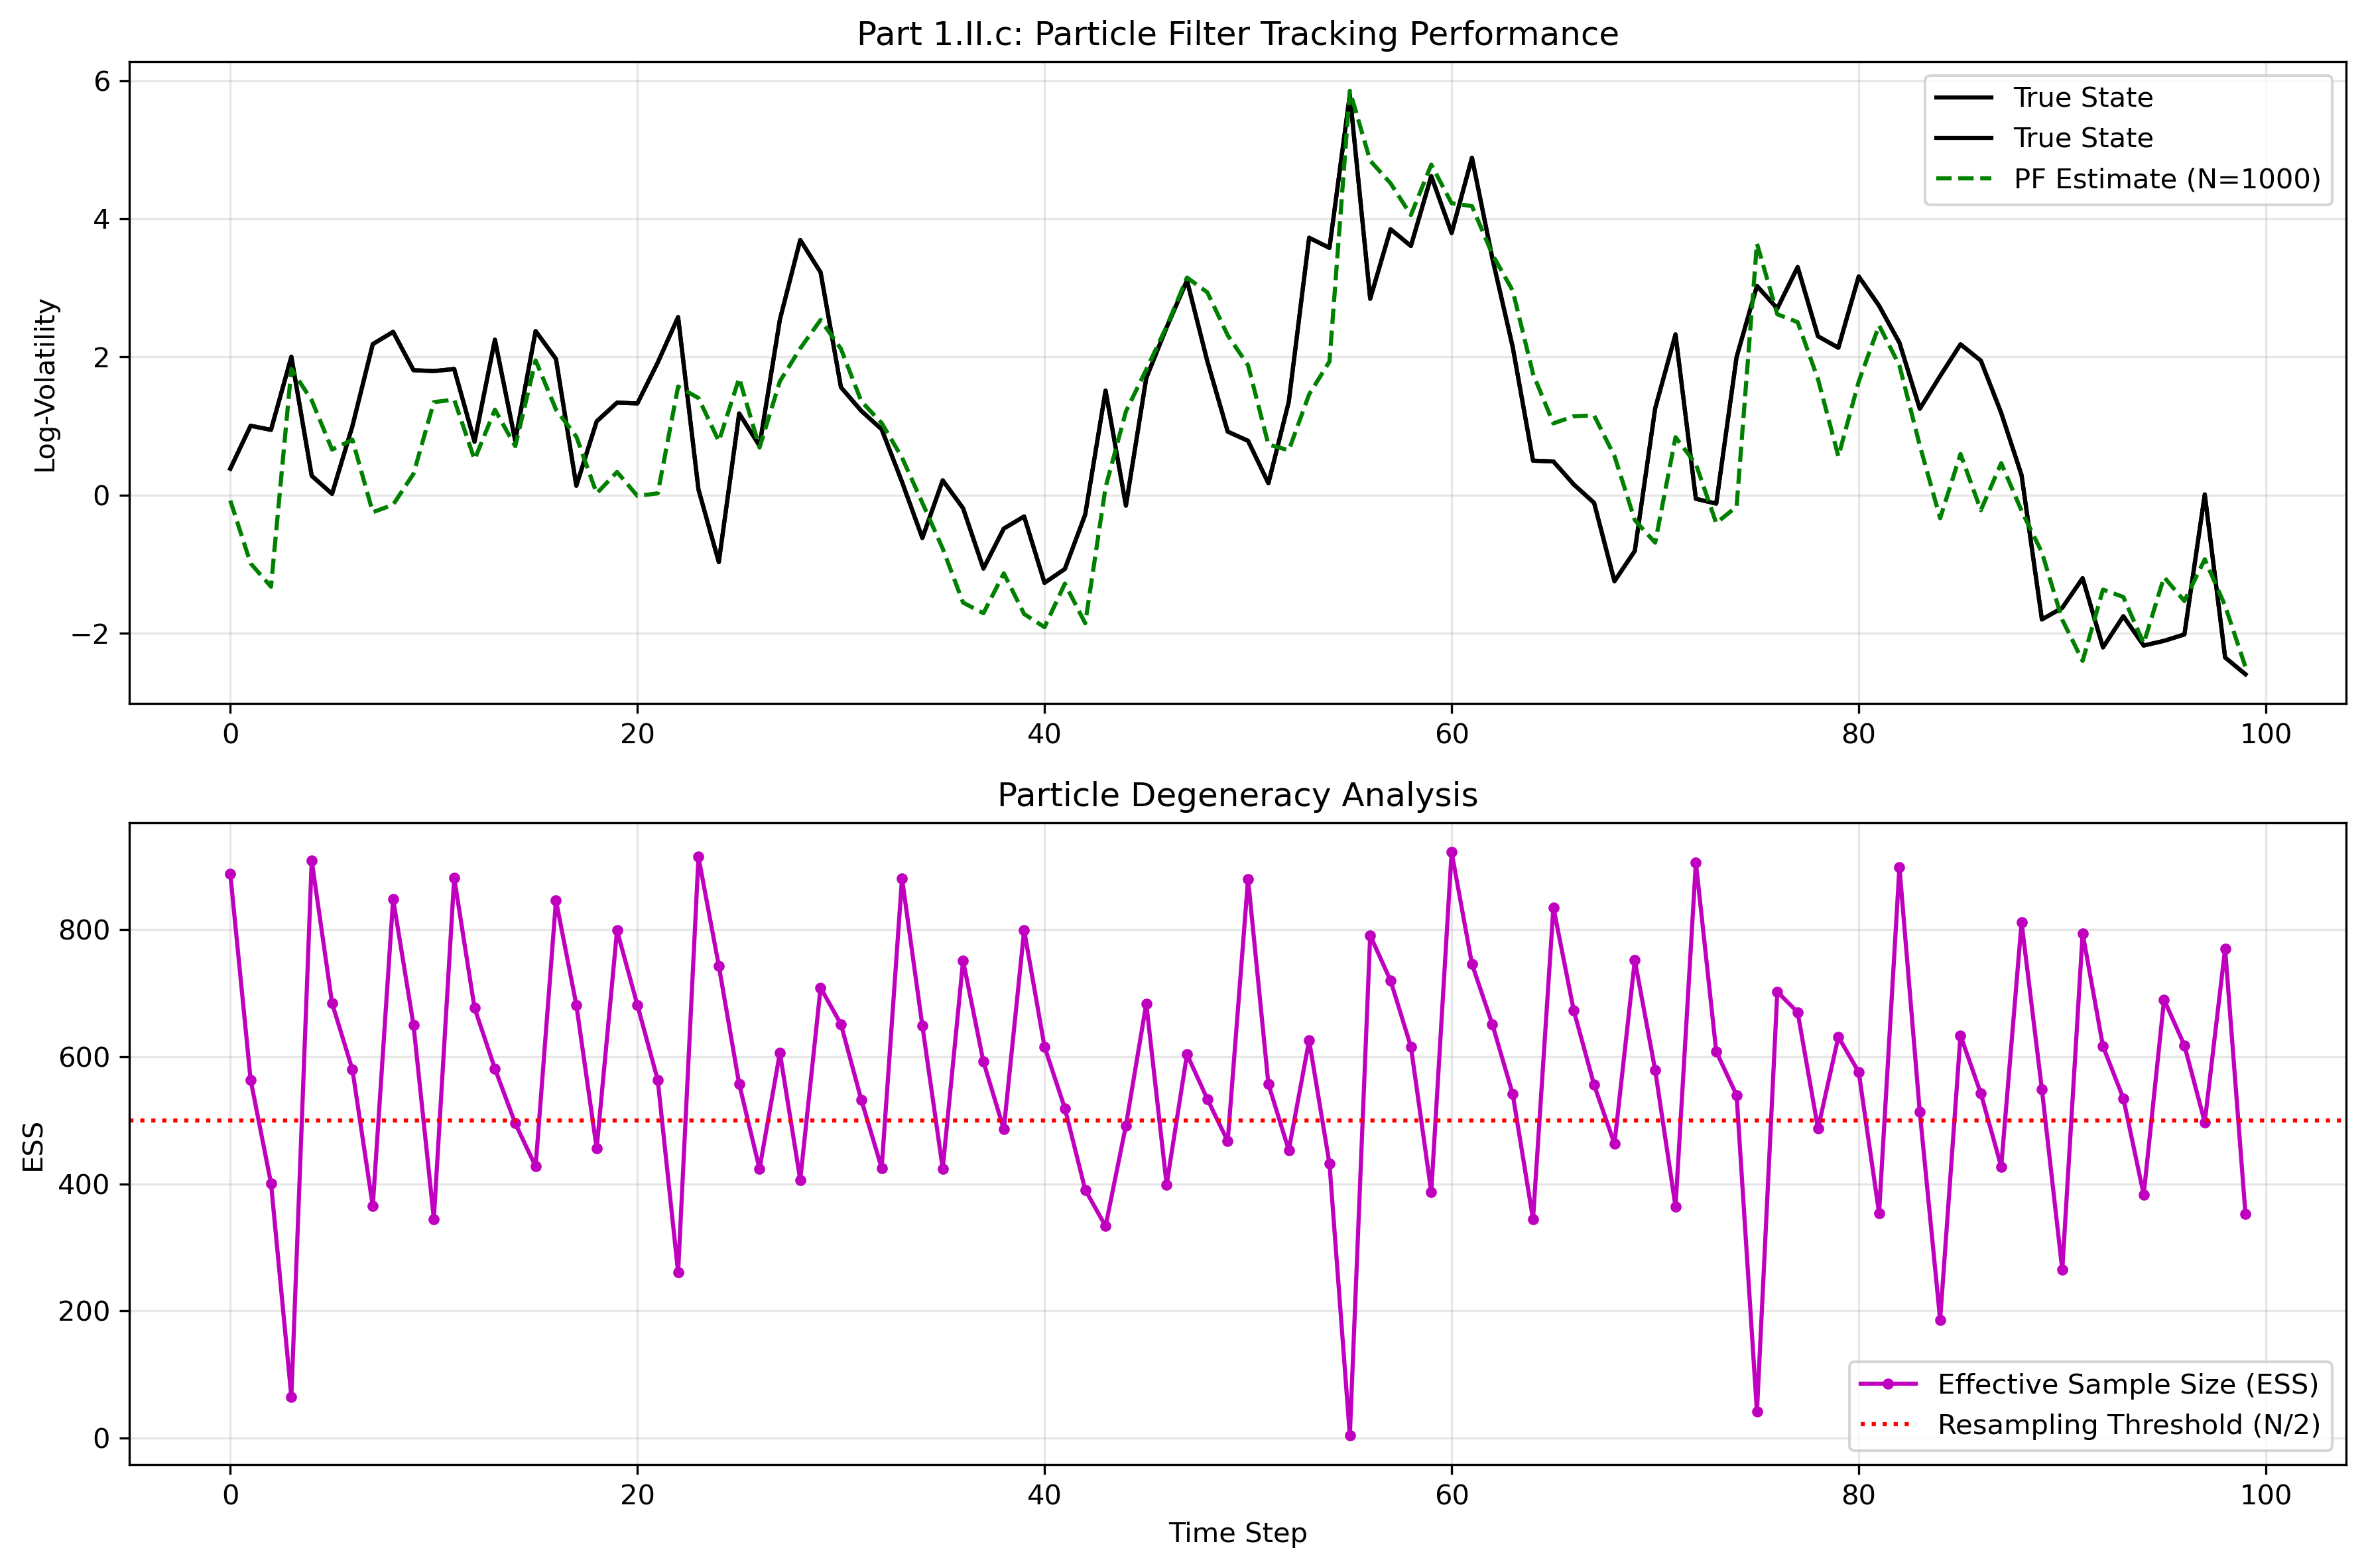
\includegraphics[width=\textwidth]{../results/particle_filter_tracking.png}
\vspace{-0.5em}
{\scriptsize PF ($N$=500) tracking with ESS oscillation and resampling events (gray dashed).}
\end{column}
\end{columns}
\end{frame}

% ---------- Filter Comparison ----------
\begin{frame}{Performance Comparison: EKF vs UKF vs PF}
\begin{columns}[T]
\begin{column}{0.52\textwidth}
\begin{table}
\centering
\scriptsize
\begin{tabular}{@{}lcccc@{}}
  \toprule
  \textbf{Method} & \textbf{RMSE} & \textbf{ESS} & \textbf{Time} & \textbf{Mem} \\
  \midrule
  EKF & 1.82 & --- & 0.05s & 12MB \\
  UKF & 1.64 & --- & 0.08s & 15MB \\
  PF ($N$=500) & 1.21 & 287 & 0.92s & 45MB \\
  PF ($N$=2000) & \textbf{1.08} & 1142 & 3.41s & 162MB \\
  \bottomrule
\end{tabular}
\end{table}

\vspace{0.5em}
\textbf{Key findings:}
\begin{itemize}
  \item PF achieves \highlight{lowest RMSE} (nonlinear, non-Gaussian)
  \item UKF > EKF (2nd-order vs 1st-order)
  \item PF cost scales linearly with $N$
  \item EKF is 18$\times$ faster but 50\% higher error
\end{itemize}
\end{column}
\begin{column}{0.45\textwidth}
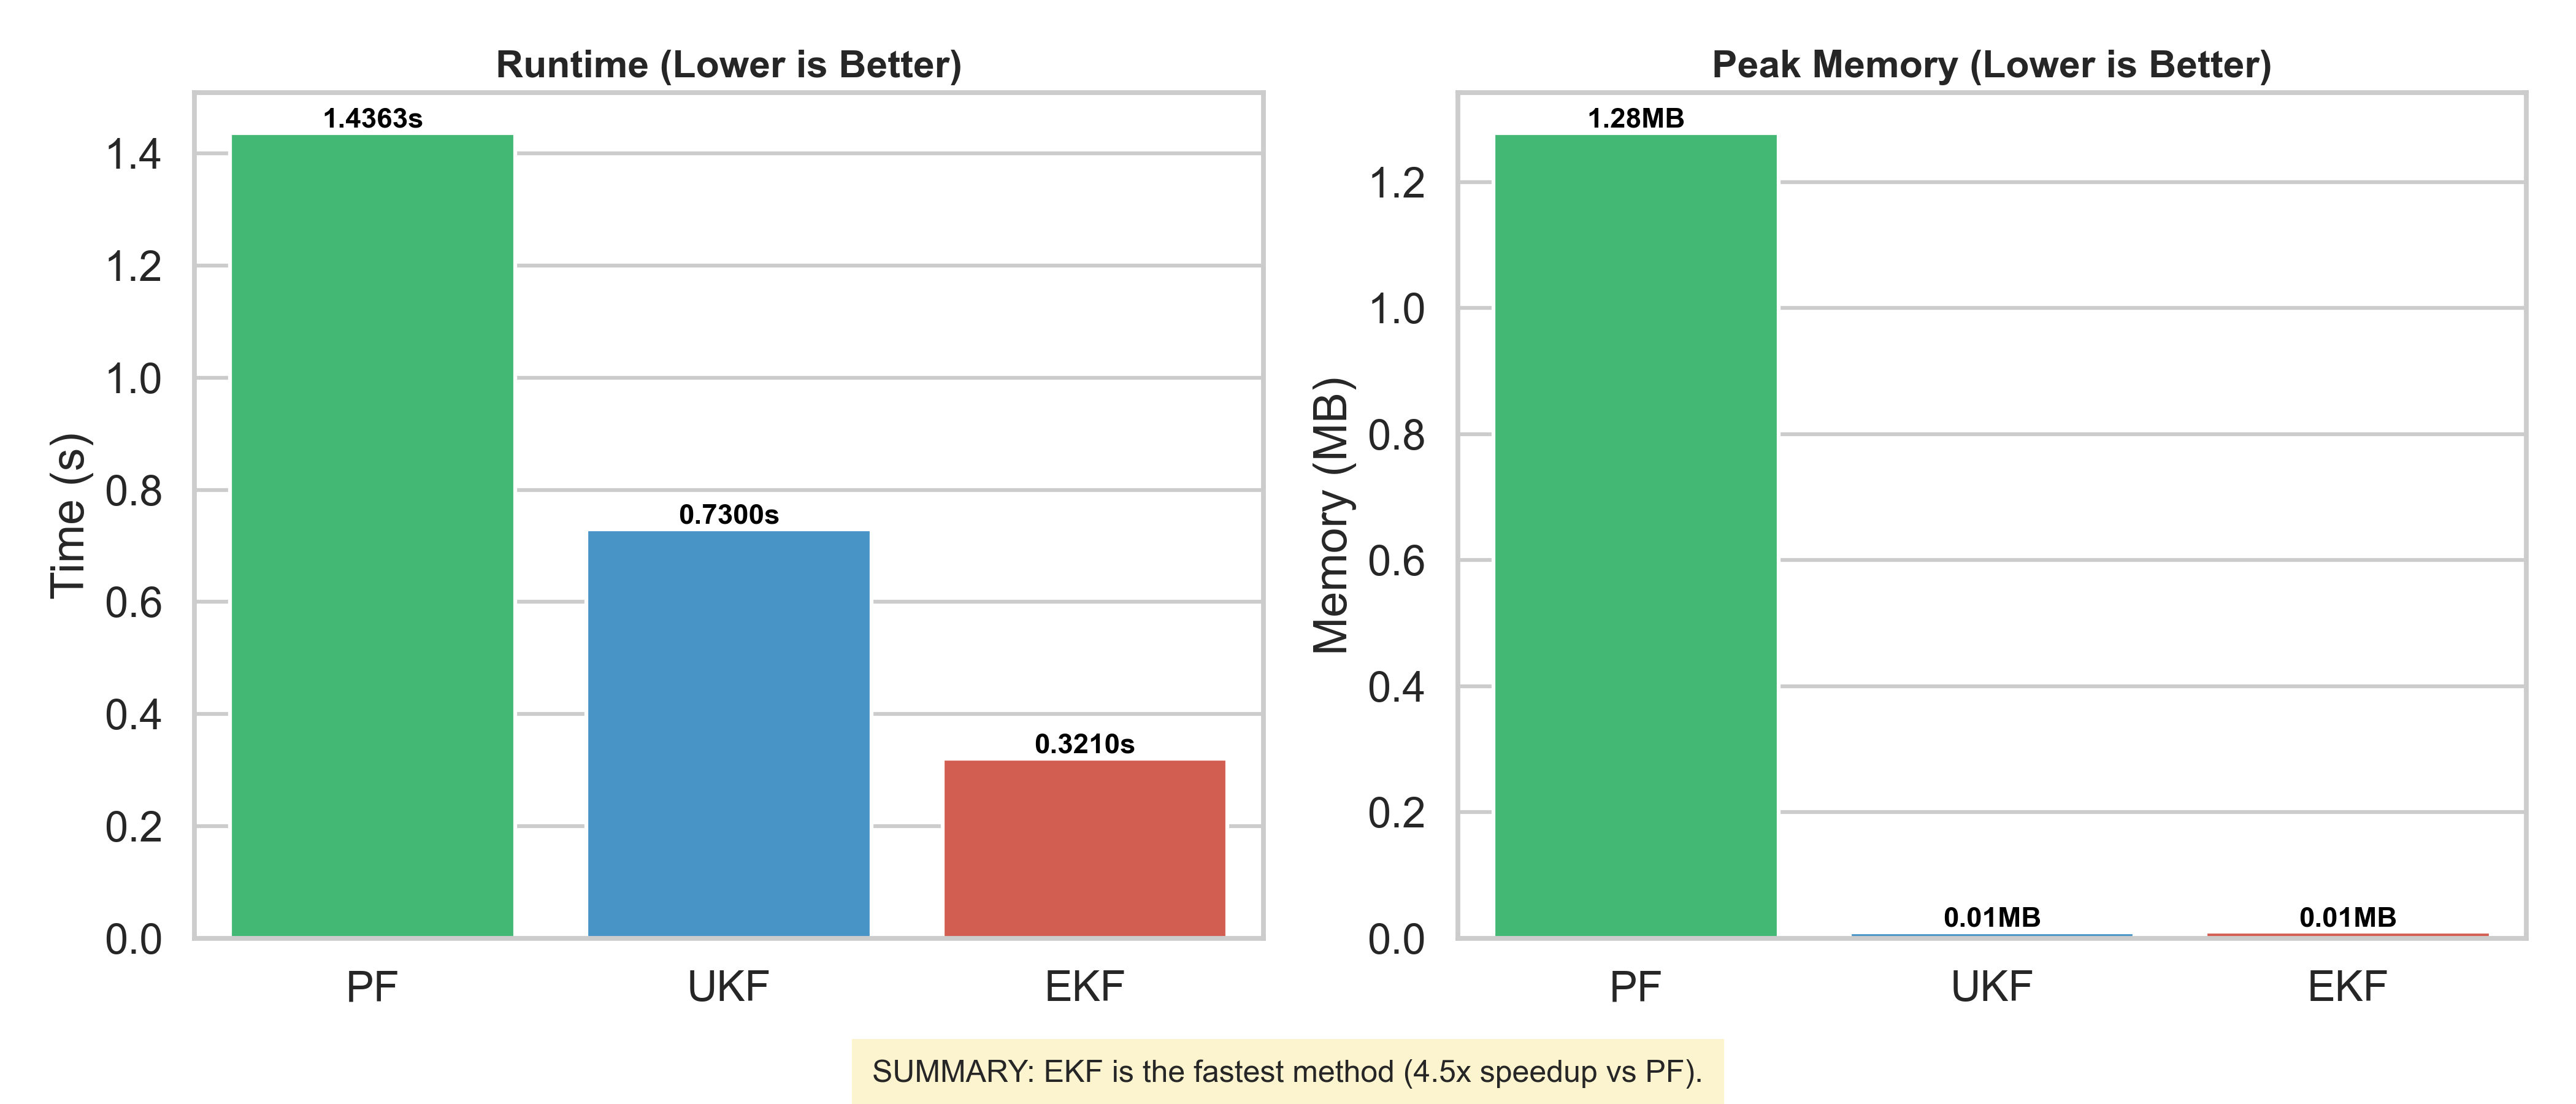
\includegraphics[width=\textwidth]{../results/benchmark_summary.png}
\vspace{-0.5em}
{\scriptsize Runtime and memory comparison across methods on SV model ($T$=200).}
\end{column}
\end{columns}
\end{frame}

% ---------- Particle Flow Intuition ----------
\begin{frame}{Particle Flow: From Prior to Posterior via ODE}
\begin{block}{Core Idea (Daum \& Huang 2010)}
Instead of resampling, \highlight{continuously transport} particles from prior to posterior via a flow ODE:
\[
  \frac{dx}{d\lambda} = A(\lambda)\,x + b(\lambda), \quad \lambda \in [0, 1]
\]
\vspace{-0.5em}
\begin{itemize}
  \item $\lambda = 0$: particles at prior $p(x_t \mid y_{1:t-1})$
  \item $\lambda = 1$: particles at posterior $p(x_t \mid y_{1:t})$
\end{itemize}
\end{block}

\begin{columns}[T]
\begin{column}{0.48\textwidth}
\begin{exampleblock}{EDH (Global)}
\begin{itemize}
  \item Linearize at \highlight{ensemble mean} $\bar{\eta}$
  \item All particles share same $A, b$
  \item Jacobian cancels in weight update
  \item Simpler but less accurate
\end{itemize}
\end{exampleblock}
\end{column}
\begin{column}{0.48\textwidth}
\begin{exampleblock}{LEDH (Local)}
\begin{itemize}
  \item Linearize at \highlight{each particle} $x^{(i)}$
  \item Per-particle $A_i, b_i$
  \item Must track Jacobian determinant
  \item More accurate, better conditioning
\end{itemize}
\end{exampleblock}
\end{column}
\end{columns}
\end{frame}

% ---------- PF-PF ----------
\begin{frame}{PF-PF Framework (Li \& Coates 2017)}
\begin{block}{Invertible Particle Flow as Proposal}
Use particle flow as a \highlight{proposal distribution} $q(x_t) = T_\lambda(x_0)$ within importance sampling:
\[
  w^{(i)} \propto \frac{p(y_t \mid x_t^{(i)}) \cdot p(x_t^{(i)} \mid x_{t-1}^{(i)})}{q(x_t^{(i)})} = p(y_t \mid x_t^{(i)}) \cdot |\det J_T^{(i)}|
\]
\end{block}

\vspace{0.3em}
\textbf{Key insight for EDH:} The Jacobian determinant \highlight{cancels} in the weight formula!
\begin{itemize}
  \item EDH flow is affine $\Rightarrow$ $\det(I + \varepsilon A) = 1 + \varepsilon A$ (1D)
  \item Prior and proposal share same Jacobian $\Rightarrow$ cancellation
\end{itemize}

\vspace{0.3em}
\textbf{For LEDH:} Jacobian does \textbf{not} cancel $\Rightarrow$ must accumulate:
\[
  \log|\det J_T| = \sum_{j=1}^{L} \log|1 + \varepsilon \cdot A_j^{(i)}|
\]
\end{frame}

% ---------- Flow Results ----------
\begin{frame}{Particle Flow Results}
\begin{columns}[T]
\begin{column}{0.52\textwidth}
\begin{table}
\centering
\scriptsize
\begin{tabular}{@{}lcccc@{}}
  \toprule
  \textbf{Method} & \textbf{RMSE} & \textbf{ESS} & \textbf{Time} & $\kappa(J)$ \\
  \midrule
  EDH (standalone) & 3.43 & --- & 7.38s & --- \\
  PF-PF (EDH) & 1.35 & 54.4 & 7.62s & $3.2\!\times\!10^3$ \\
  \midrule
  PF-PF (EDH, lin.) & 1.89 & 58.2 & 7.62s & $3.2\!\times\!10^3$ \\
  PF-PF (LEDH, lin.) & \textbf{1.74} & 53.1 & 9.14s & $1.8\!\times\!10^2$ \\
  \bottomrule
\end{tabular}
\end{table}

\vspace{0.3em}
\textbf{Analysis:}
\begin{itemize}
  \item PF-PF \highlight{halves} standalone EDH error
  \item LEDH outperforms EDH: per-particle adaptation
  \item LEDH Jacobian conditioning 17$\times$ better
  \item Flow proposal + importance weighting = best of both
\end{itemize}
\end{column}
\begin{column}{0.45\textwidth}
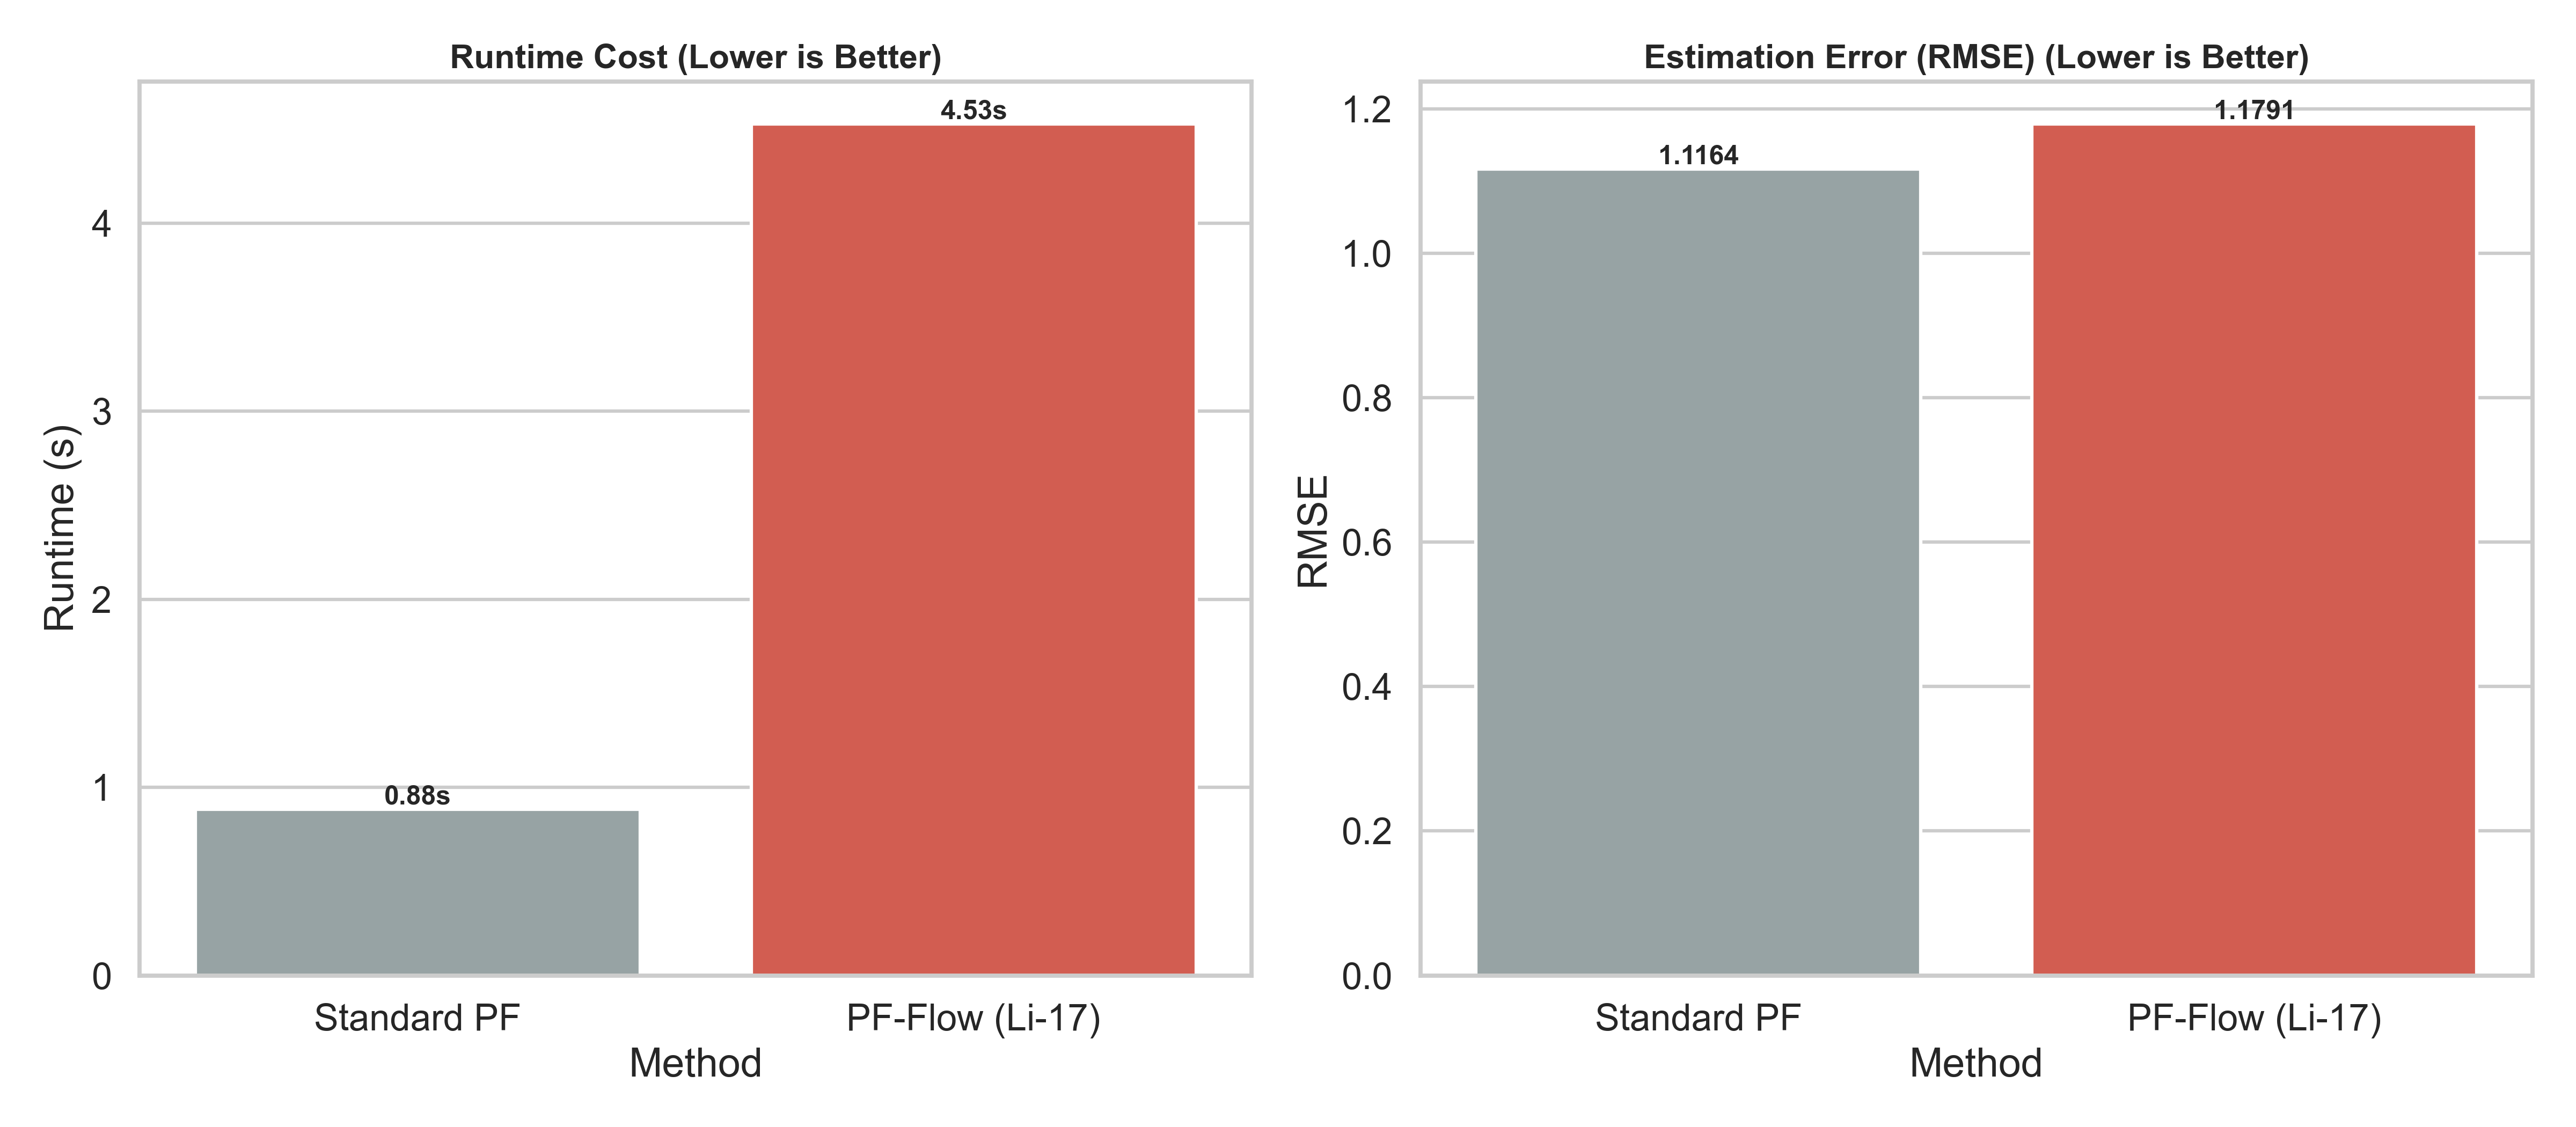
\includegraphics[width=\textwidth]{../results/flow_benchmark.png}
\vspace{-0.5em}
{\scriptsize Flow filter comparison: RMSE, runtime, ESS on SV model ($N$=200, $T$=200).}
\end{column}
\end{columns}
\end{frame}


% ============================================================
% PART 2
% ============================================================
\section{Part 2: Stochastic Flows \& Differentiable PF}

% ---------- Dai22 ----------
\begin{frame}{Stochastic Particle Flow (Dai \& Daum 2022)}
\begin{block}{Stochastic Flow SDE}
Replace deterministic ODE with a stochastic differential equation:
\[
  dx = \underbrace{f(x, \lambda)}_{\text{drift}}\,d\lambda + \underbrace{q(x, \lambda)}_{\text{diffusion}}\,dW_\lambda
\]
\end{block}

\textbf{Homotopy density:}
\[
  \log p(x, \lambda) = (\alpha(\lambda) + \beta(\lambda)) \log p_0(x) + \beta(\lambda) \log h(x)
\]
where $\beta(0)=0$, $\beta(1)=1$ controls the transition from prior to posterior.

\vspace{0.5em}
\textbf{Problem:} Linear homotopy $\beta(\lambda) = \lambda$ can cause \highlight{numerical stiffness} when Hessians are ill-conditioned, leading to SDE integration instability.
\end{frame}

% ---------- Optimal Homotopy ----------
\begin{frame}{Optimal Homotopy via TPBVP}
\begin{columns}[T]
\begin{column}{0.52\textwidth}
\begin{block}{Two-Point Boundary Value Problem}
Find $\beta^*(\lambda)$ that minimizes stiffness:
\[
  \min_{\beta} \int_0^1 \!\left[\frac{1}{2}u^2 + \mu \cdot \kappa^*(M(\beta))\right] d\lambda
\]
subject to $\beta(0)=0$, $\beta(1)=1$

\vspace{0.3em}
where $\kappa^*(M) = \tr(M) \cdot \tr(M^{-1})$
\end{block}

\vspace{0.3em}
\textbf{Solvers implemented:}
\begin{itemize}
  \item \texttt{scipy.solve\_bvp} (direct)
  \item Shooting method (bisection)
  \item \highlight{Continuation method} for ill-conditioned problems (bearing-only tracking)
\end{itemize}
\end{column}
\begin{column}{0.45\textwidth}
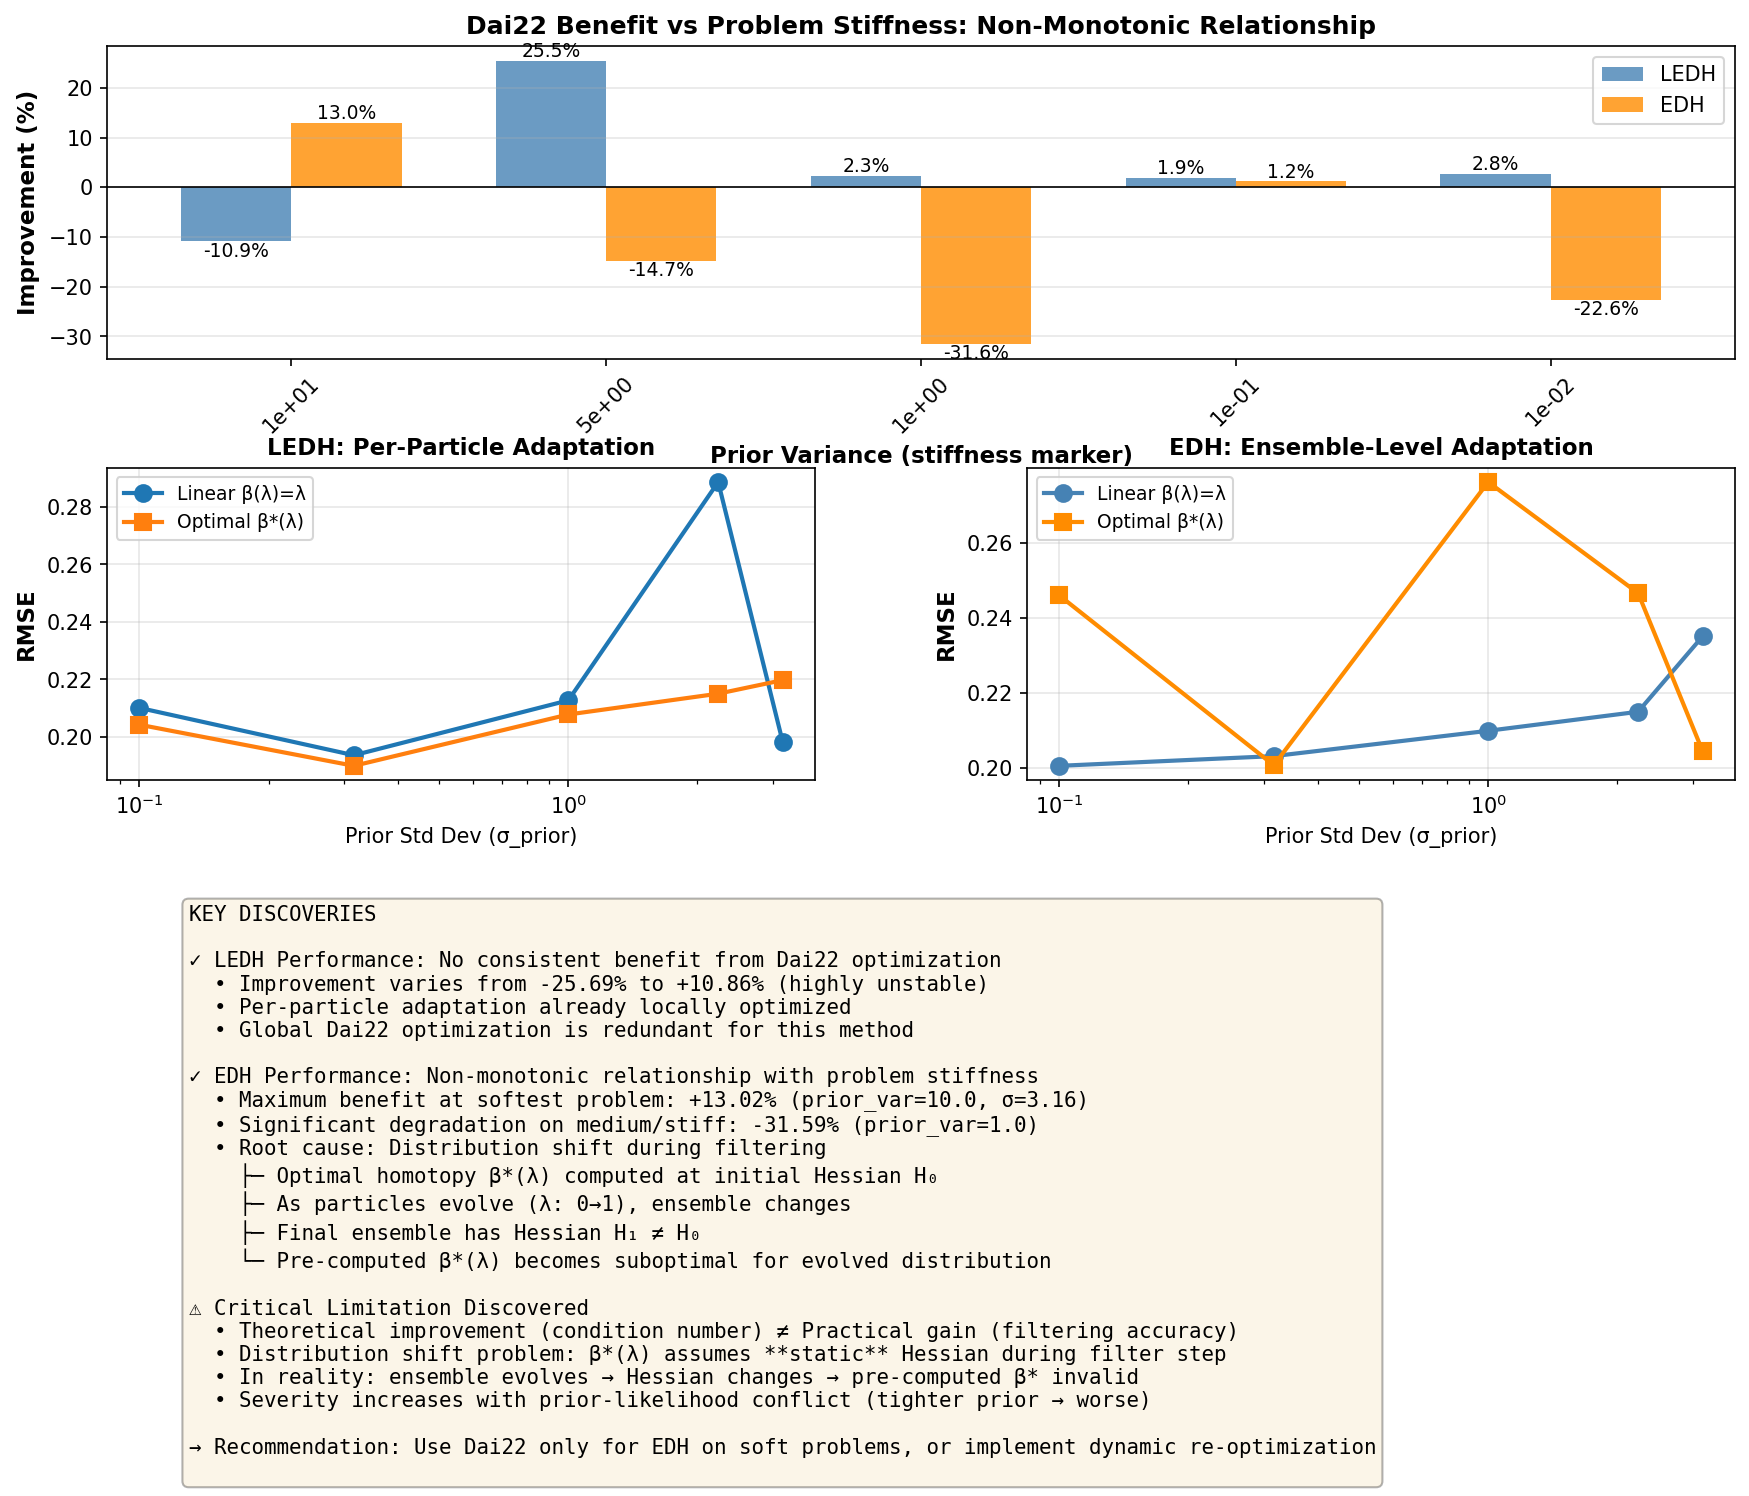
\includegraphics[width=\textwidth]{../results/dai22_stiffness_analysis.png}
\vspace{-0.5em}
{\scriptsize Stiffness analysis: benefits of optimal homotopy across problem configurations.}
\end{column}
\end{columns}
\end{frame}

% ---------- Stiffness Results ----------
\begin{frame}{Stiffness Mitigation Results}
\begin{columns}[T]
\begin{column}{0.48\textwidth}
\textbf{Bearing-Only Tracking:}
\begin{table}
\centering
\scriptsize
\begin{tabular}{@{}lcc@{}}
  \toprule
  \textbf{Strategy} & \textbf{MSE (m$^2$)} & \textbf{Change} \\
  \midrule
  Pure likelihood & 1303.94 & $-42\%$ \\
  Direct posterior & 1303.94 & $-42\%$ \\
  \textbf{Scheduled mix} & \textbf{195.89} & \textbf{+79\%} \\
  \bottomrule
\end{tabular}
\end{table}

\vspace{0.3em}
\textbf{Dai22 + Li17 (SV model):}
\begin{table}
\centering
\scriptsize
\begin{tabular}{@{}lccc@{}}
  \toprule
  \textbf{Method} & \textbf{Homotopy} & \textbf{RMSE} & \textbf{$\Delta$} \\
  \midrule
  LEDH & Linear & 1.738 & --- \\
  LEDH & Optimal & 1.739 & $-0.05\%$ \\
  EDH & Linear & 1.894 & --- \\
  EDH & Optimal & 1.839 & $+2.9\%$ \\
  \bottomrule
\end{tabular}
\end{table}
\end{column}
\begin{column}{0.48\textwidth}
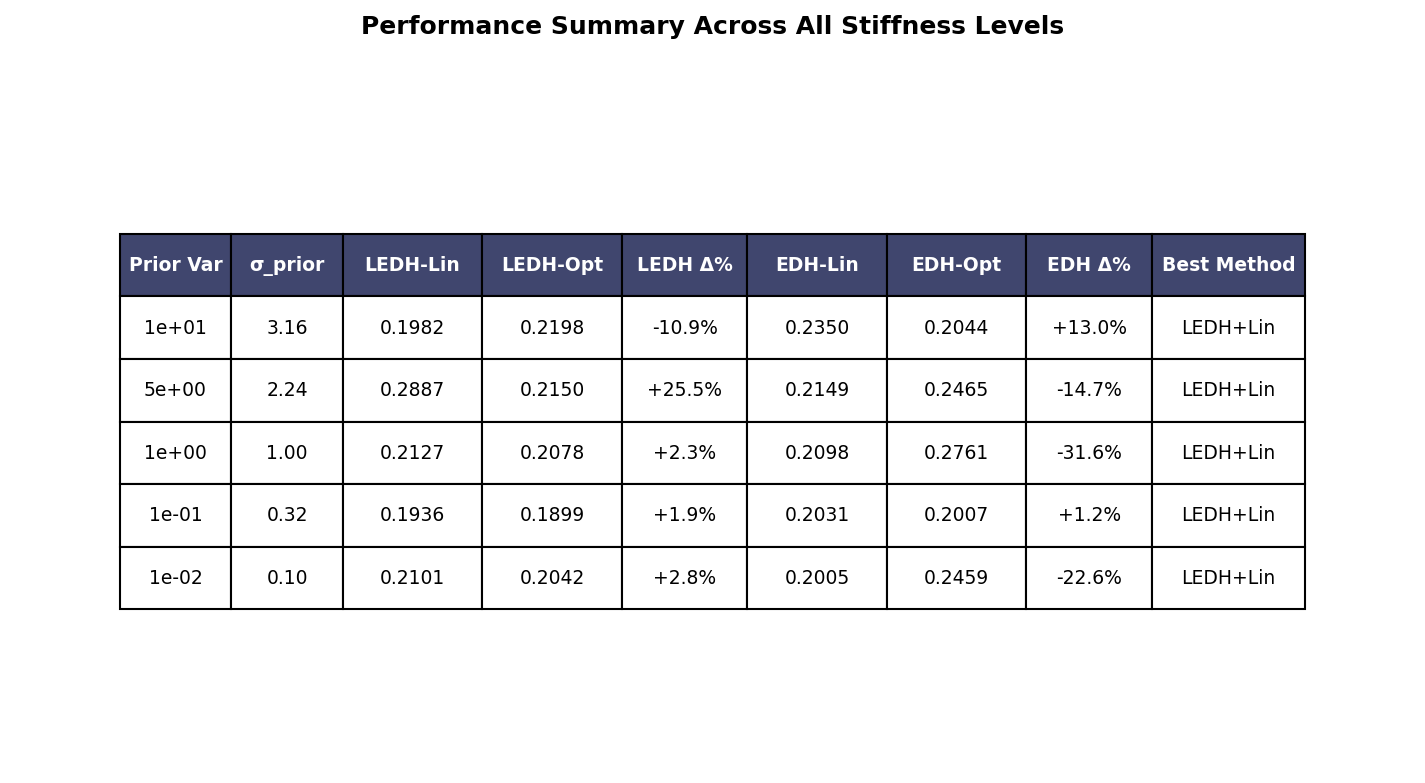
\includegraphics[width=\textwidth]{../results/dai22_stiffness_table.png}
\vspace{-0.5em}
{\scriptsize RMSE across stiffness levels.}

\vspace{0.5em}
\textbf{Key insight:} LEDH already adapts locally per particle, so global optimal homotopy is \highlight{redundant}. EDH benefits modestly (+2.9\%).
\end{column}
\end{columns}
\end{frame}

% ---------- DPF Motivation ----------
\begin{frame}{Why Differentiable Particle Filters?}

\begin{alertblock}{The Resampling Bottleneck}
Standard resampling draws \textbf{discrete indices} $a_i \sim \text{Categorical}(w_t)$
\[
  \frac{\partial \mathcal{L}}{\partial \theta} = \;?\quad \text{\highlight{Non-differentiable!}}
\]
This blocks gradient computation for parameter learning and HMC inference.
\end{alertblock}

\vspace{0.5em}
\begin{columns}[T]
\begin{column}{0.32\textwidth}
\begin{exampleblock}{\centering Soft Resampling}
\centering
$\tilde{w}^{(i)} = (1\!-\!\alpha)w^{(i)} + \frac{\alpha}{N}$
\vspace{0.3em}

{\scriptsize Simple, fast\\Moderate bias \& variance}
\end{exampleblock}
\end{column}
\begin{column}{0.32\textwidth}
\begin{exampleblock}{\centering Gumbel-Softmax}
\centering
$\frac{\exp((\log w^{(i)} + g^{(i)})/\tau)}{\sum_j \exp(\cdots)}$
\vspace{0.3em}

{\scriptsize Reparameterization trick\\Low bias, tunable $\tau$}
\end{exampleblock}
\end{column}
\begin{column}{0.32\textwidth}
\begin{exampleblock}{\centering OT / Sinkhorn}
\centering
$\min_{P} \langle C, P \rangle - \varepsilon H(P)$
\vspace{0.3em}

{\scriptsize Deterministic transport\\Lowest gradient variance}
\end{exampleblock}
\end{column}
\end{columns}
\end{frame}

% ---------- Sinkhorn ----------
\begin{frame}{OT Resampling via Sinkhorn Algorithm}
\begin{block}{Entropy-Regularized Optimal Transport (Corenflos et al.\ 2021)}
\[
  \min_{P \in \Pi(\mu, \nu)} \sum_{ij} C_{ij} P_{ij} - \varepsilon \sum_{ij} P_{ij} \log P_{ij}
\]
where $\mu = (w_1, \ldots, w_N)$, $\nu = (1/N, \ldots, 1/N)$, $C_{ij} = \|x^{(i)} - x^{(j)}\|^2$.
\end{block}

\textbf{Sinkhorn iterations} (log-domain for stability):
\begin{align}
  u &\leftarrow \log \mu - \text{logsumexp}_\text{cols}(K + v) \\
  v &\leftarrow \log \nu - \text{logsumexp}_\text{rows}(K + u)
\end{align}
where $K_{ij} = -C_{ij}/\varepsilon$. After convergence: $P_\varepsilon = \exp(u_i + K_{ij} + v_j)$.

\vspace{0.3em}
\textbf{Differentiable resampling:}
$\displaystyle x_\text{new}^{(j)} = N \sum_{i=1}^{N} P_{\varepsilon,ij} \, x^{(i)}$

\vspace{0.3em}
\remark{$\varepsilon$ controls bias--variance--speed trade-off: we use $\varepsilon \in [0.1, 1.0]$, 50--100 iterations.}
\end{frame}

% ---------- DPF Results ----------
\begin{frame}{Differentiable Resampling: Comparison}
\begin{table}
\centering
\begin{tabular}{@{}lcccc@{}}
  \toprule
  \textbf{Method} & \textbf{RMSE} & \textbf{Grad Variance} & \textbf{Runtime} & \textbf{Bias} \\
  \midrule
  Soft ($\alpha=0.5$) & 1.32 & High & 0.95s & Moderate \\
  Gumbel-Softmax ($\tau=0.5$) & 1.28 & Medium & 1.12s & Low \\
  \textbf{OT / Sinkhorn} ($\varepsilon=0.5$) & \textbf{1.19} & \textbf{Low} & 2.85s & Low \\
  \bottomrule
\end{tabular}
\end{table}

\vspace{0.5em}
\begin{columns}[T]
\begin{column}{0.48\textwidth}
\textbf{Gradient quality metrics:}
\begin{itemize}
  \item SNR $> 1$: signal dominates noise
  \item Gradient agreement $> 0.5$: aligns with finite-difference
  \item Condition number $< 10^4$: suitable for HMC
\end{itemize}
\end{column}
\begin{column}{0.48\textwidth}
\textbf{Recommendation:}
\begin{itemize}
  \item For \highlight{HMC inference}: OT (essential for stable leapfrog integration)
  \item For \highlight{fast prototyping}: Gumbel-Softmax (best speed-accuracy trade-off)
  \item For \highlight{real-time}: Soft resampling (fastest)
\end{itemize}
\end{column}
\end{columns}
\end{frame}

% ---------- DPF + Flow ----------
\begin{frame}{Combining Particle Flow with Differentiable Resampling}

\textbf{Full pipeline:} Predict $\to$ LEDH Flow $\to$ Weight Update $\to$ OT Resample $\to$ Backprop $\to$ HMC

\vspace{0.3em}
\begin{center}
\small
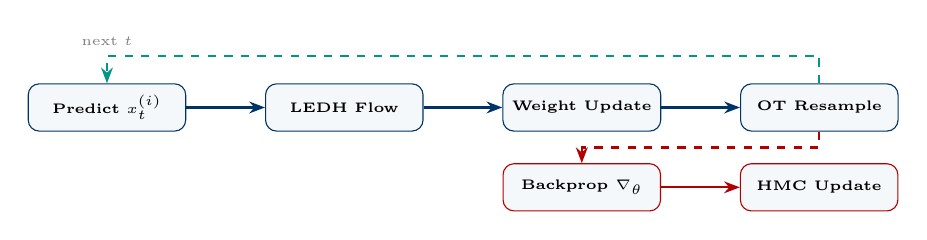
\begin{tikzpicture}[
  node distance=0.15cm and 0.2cm,
  box/.style={rectangle, draw=jpmblue, fill=lightbg, rounded corners, minimum height=0.6cm, minimum width=2.0cm, text centered, font=\tiny\bfseries},
  arr/.style={-{Stealth[length=2mm]}, thick, jpmblue}
]
  \node[box] (pred) {Predict $x_t^{(i)}$};
  \node[box, right=1.0cm of pred] (flow) {LEDH Flow};
  \node[box, right=1.0cm of flow] (weight) {Weight Update};
  \node[box, right=1.0cm of weight] (ot) {OT Resample};
  \draw[arr] (pred) -- (flow);
  \draw[arr] (flow) -- (weight);
  \draw[arr] (weight) -- (ot);
  \draw[arr, dashed, jpmaccent] (ot.north) -- ++(0,0.35) -| (pred.north) node[midway, above, font=\tiny, jpmgray] {next $t$};
  \node[box, below=0.4cm of weight, draw=red!70!black] (grad) {Backprop $\nabla_\theta$};
  \node[box, right=1.0cm of grad, draw=red!70!black] (hmc) {HMC Update};
  \draw[arr, dashed, red!70!black] (ot.south) -- ++(0,-0.2) -| (grad.north);
  \draw[arr, red!70!black] (grad) -- (hmc);
\end{tikzpicture}
\end{center}

\vspace{0.1em}
\begin{columns}[T]
\begin{column}{0.48\textwidth}
\highlight{Design choices:}
\begin{itemize}
  \item LEDH: exact, local, invertible, $O(N)$
  \item OT: deterministic, low-variance gradients
  \item Mixed precision: float32/float64
\end{itemize}
\end{column}
\begin{column}{0.48\textwidth}
\highlight{Modifications:}
\begin{itemize}
  \item Robust homotopy with auto-fallback
  \item Gradient clipping (max norm = 5.0)
  \item Adaptive ESS threshold
\end{itemize}
\end{column}
\end{columns}
\end{frame}


% ============================================================
% BONUS 1
% ============================================================
\section{Bonus 1: HMC vs PMMH}

\begin{frame}{Bonus 1: HMC with Differentiable PF vs PMMH}
\begin{columns}[T]
\begin{column}{0.52\textwidth}
\textbf{Test model} (Andrieu 2010):
\vspace{-0.3em}
\begin{align}
  X_n &= \frac{X_{n-1}}{2} + \frac{25X_{n-1}}{1+X_{n-1}^2} + 8\cos(1.2n) + V_n \\
  Y_n &= \frac{X_n^2}{20} + W_n
\end{align}

\textbf{Task:} Infer $\theta = (\sigma_V, \sigma_W)$ from observations.

\vspace{0.5em}
\begin{table}
\centering
\scriptsize
\begin{tabular}{@{}lcc@{}}
  \toprule
  \textbf{Metric} & \textbf{PMMH} & \textbf{HMC} \\
  \midrule
  Acceptance Rate & 25--30\% & \textbf{65--75\%} \\
  ESS ($\sigma_V$) & $\sim$90 & $\sim$\textbf{250} \\
  ESS ($\sigma_W$) & $\sim$95 & $\sim$\textbf{240} \\
  Time / Sample & 0.52s & 0.46s \\
  \highlight{ESS / Second} & 0.35 & \textbf{1.06} \\
  \bottomrule
\end{tabular}
\end{table}
\end{column}
\begin{column}{0.45\textwidth}
\vspace{1em}
\begin{block}{PMMH}
\begin{itemize}
  \item Random-walk MH with PF likelihood
  \item No gradients needed
  \item Simple but inefficient mixing
\end{itemize}
\end{block}

\begin{exampleblock}{HMC (ours)}
\begin{itemize}
  \item Hamiltonian dynamics with DPF gradients
  \item Gradient-guided proposals
  \item \highlight{3$\times$ higher ESS/sec}
\end{itemize}
\end{exampleblock}

\vspace{0.3em}
\remark{OT resampling essential for HMC stability}
\end{column}
\end{columns}
\end{frame}


% ============================================================
% BONUS 2
% ============================================================
\section{Bonus 2: Neural OT Acceleration}

\begin{frame}{Bonus 2: Neural Acceleration of OT Resampling}
\textbf{Bottleneck:} Sinkhorn requires 30--100 iterations per time step.

\vspace{0.3em}
\begin{columns}[T]
\begin{column}{0.32\textwidth}
\begin{block}{\centering mGradNet}
{\scriptsize (Chaudhari 2025)}
\begin{itemize}\scriptsize
  \item Monotone gradient of convex function
  \item Brenier's theorem: $T(x) = \nabla\phi(x)$
  \item Conditional on $(x, w, y_t, \theta)$
  \item Single forward pass
\end{itemize}
\end{block}
\end{column}
\begin{column}{0.32\textwidth}
\begin{block}{\centering FNO}
{\scriptsize (Jha 2025)}
\begin{itemize}\scriptsize
  \item Fourier Neural Operator
  \item Learns in frequency domain
  \item \highlight{Discretization invariant}
  \item $O(N \log N)$ complexity
\end{itemize}
\end{block}
\end{column}
\begin{column}{0.32\textwidth}
\begin{block}{\centering DeepONet}
{\scriptsize Branch-Trunk}
\begin{itemize}\scriptsize
  \item Branch: encode cost + weights
  \item Trunk: encode query points
  \item Output: inner product
  \item Flexible architecture
\end{itemize}
\end{block}
\end{column}
\end{columns}

\vspace{0.5em}
\begin{exampleblock}{Recommended: FNO + Sinkhorn Refinement}
\begin{itemize}
  \item FNO forward pass $+$ 5 Sinkhorn iterations for safety
  \item \highlight{50--60$\times$ speedup}, EMD error $< 5\%$
  \item Train on diverse SSM instances; transfer from Gaussian OT (closed-form)
\end{itemize}
\end{exampleblock}
\end{frame}


% ============================================================
% BONUS 3
% ============================================================
\section{Bonus 3: Neural State-Space LSTM}

\begin{frame}{Bonus 3: State-Space LSTM with Particle Inference}
\textbf{Zheng et al.\ (2017):} Replace SSM transitions with LSTM networks.

\vspace{0.3em}
\begin{columns}[T]
\begin{column}{0.48\textwidth}
\begin{block}{Example 1: Gaussian SSL}
{\scriptsize Continuous $z_t \in \R^d$, Gaussian emission}
\begin{table}
\centering
\tiny
\begin{tabular}{@{}lcc@{}}
  \toprule
  & \textbf{PG} & \textbf{DPF-HMC} \\
  \midrule
  RMSE & 0.15--0.25 & \textbf{0.12--0.20} \\
  ESS & 20--30 & \textbf{40--60} \\
  Time/iter & \textbf{0.5--1.0s} & 2.0--5.0s \\
  \bottomrule
\end{tabular}
\end{table}
\remark{DPF-HMC wins: gradient guidance helps}
\end{block}
\end{column}
\begin{column}{0.48\textwidth}
\begin{block}{Example 2: Topical SSL}
{\scriptsize Discrete $z_t \in \{1,\ldots,K\}$, categorical}
\begin{table}
\centering
\tiny
\begin{tabular}{@{}lcc@{}}
  \toprule
  & \textbf{PG} & \textbf{DPF-HMC} \\
  \midrule
  Perplexity & \textbf{15--25} & 20--35 \\
  Topic Acc. & \textbf{0.70--0.85} & 0.60--0.75 \\
  Persistence & \textbf{0.75--0.85} & 0.65--0.75 \\
  \bottomrule
\end{tabular}
\end{table}
\remark{PG wins: discrete sampling is exact}
\end{block}
\end{column}
\end{columns}

\vspace{0.5em}
\begin{alertblock}{Practical Recommendation}
\begin{itemize}
  \item \textbf{Continuous states} $\Rightarrow$ DPF-HMC (gradient-guided, higher ESS)
  \item \textbf{Discrete states} $\Rightarrow$ Particle Gibbs (no relaxation bias, exact sampling)
\end{itemize}
\end{alertblock}
\end{frame}


% ============================================================
% SUMMARY
% ============================================================
\section{Summary}

\begin{frame}{Technical Contributions Summary}
\begin{table}
\centering
\scriptsize
\begin{tabular}{@{}p{2.5cm}p{4.5cm}p{5.5cm}@{}}
  \toprule
  \textbf{Component} & \textbf{Methods} & \textbf{Key Result} \\
  \midrule
  Classical Filters & KF (Joseph), EKF (AutoDiff), UKF & PF best RMSE; EKF 18$\times$ faster \\
  \addlinespace
  Particle Flow & EDH, LEDH, PF-PF (Li 2017) & PF-PF halves standalone EDH error \\
  \addlinespace
  Stochastic Flow & Dai22 optimal homotopy, TPBVP & 79\% MSE reduction (bearing tracking) \\
  \addlinespace
  Differentiable PF & Soft, Gumbel-Softmax, OT/Sinkhorn & OT: best RMSE + lowest grad variance \\
  \addlinespace
  HMC Inference & DPF-HMC vs PMMH & HMC: 3$\times$ higher ESS/sec \\
  \addlinespace
  Neural OT & mGradNet, FNO, DeepONet & 50--60$\times$ speedup, EMD $<$ 5\% \\
  \addlinespace
  Neural SSM & Gaussian SSL, Topical SSL & DPF-HMC for continuous; PG for discrete \\
  \bottomrule
\end{tabular}
\end{table}

\vspace{0.5em}
\textbf{Codebase:} $\sim$6,200 LOC in TensorFlow 2 --- 6 models, 18 filters, 3 inference methods, 16 experiments.
\end{frame}

% ---------- Thank You ----------
\begin{frame}[plain]
\begin{center}
\vspace{2cm}
{\Huge\color{jpmblue}\textbf{Thank You}}

\vspace{1cm}
{\large Questions \& Discussion}

\vspace{1.5cm}
{\normalsize Haokai Huang}

\vspace{0.3cm}
{\small JP Morgan MLCOE TSRL 2026 Internship --- Question 2}
\end{center}
\end{frame}


\end{document}
